\documentclass[11pt]{article}
\usepackage[margin=1in]{geometry}
\usepackage[T1]{fontenc}
\usepackage{graphicx}
\usepackage[numbers]{natbib}
\usepackage{hyperref}
\setlength{\parskip}{0.5em}
\setlength{\parindent}{0pt}

\title{What are the foundational architectures and training objectives that modern vision-language models are built on?}
\author{GraphIV --- deep research}
\date{\today}

\begin{document}
\maketitle

\begin{abstract}
The review is well-structured and covers recent trends, but it misses the most critical, high-impact foundational papers that define the field's core architectures.
\end{abstract}

\section{From Semantic Alignment to Generative Agents: A Survey of Vision-Language Architectures and Objectives}

The integration of visual perception and linguistic reasoning represents one of the most significant challenges in modern artificial intelligence. The fundamental problem lies in bridging the gap between disparate modalities—the continuous, high-dimensional nature of pixels and the discrete, symbolic nature of language. Solving this requires not only massive datasets but also the development of specialized architectures and training objectives capable of capturing complex cross-modal relationships. As vision-language models evolve from narrow tools into general-purpose reasoning engines, understanding the historical and structural shifts that have enabled this progress is essential for comprehending the current state of multimodal intelligence.

This review traces the technological trajectory of vision-language modeling, beginning with the early foundations of visual-semantic alignment and task-specific architectures. We then examine the transformative shift brought about by the rise of Transformers, which enabled unified representations through cross-modal pre-training, and the subsequent era of scaling and bootstrapping driven by contrastive learning and large-scale alignment. The discussion then moves into the recent paradigm shift of instruction tuning and the emergence of multimodal large language models. Finally, we survey the current frontier of the field, investigating the move toward high-resolution perception and the development of unified generative agents.

\subsection{Early Foundations: Visual-Semantic Alignment and Task-Specific Architectures}

The evolution of modern vision-language models is rooted in the development of large-scale datasets and the transition from simple classification to complex multimodal alignment. Early efforts focused on providing the necessary data density for sophisticated reasoning. The Microsoft COCO dataset (\citep{1405.0312}) introduced a significant shift by providing context-rich images with an average of 7.7 instances per image, supporting tasks like per-instance segmentation and relationship characterization. While COCO provided a robust multi-stage pipeline for high-quality segmentations, its focus on "thing" categories—explicitly excluding "stuff" like sky or grass—constrained its ability to model holistic environmental context (\citep{1405.0312}). This need for dense, relational data was further addressed by Visual Genome (\citep{1602.07332}), which connected language and vision through dense annotations including attribute prediction and relationship recognition.

Architectural foundations progressed from standard convolutional neural networks (CNNs) used for object category classification (\citep{1409.0575}) to deep residual learning frameworks (ResNet) that enabled more effective training of deep networks for detection and segmentation (\citep{1512.03385}). These visual backbones were then integrated with linguistic components to achieve semantic alignment. One early approach utilized a two-stage learning paradigm to align sentence snippets with visual regions through a multimodal embedding, combining CNNs and bidirectional RNNs (\citep{1412.2306}). Similarly, the Multimodal Skip-gram model (\citep{1501.02598}) employed a self-supervised learning paradigm to jointly predict linguistic contexts and visual features using a softmax objective.

As tasks became more specialized, architectures evolved to handle specific modalities of interaction:

\begin{itemize}
  \item   \textbf{Referring Expressions:} To move beyond simple labeling, models like those in \citep{1511.02283} and \citep{1608.00272} utilized CNN-LSTM architectures. These models augmented visual representations with region-of-interest features and location information to facilitate both referring expression generation and comprehension.
  \item   \textbf{Visual Question Answering (VQA):} The introduction of VQA (\citep{1505.00468}) shifted the focus toward open-ended reasoning. However, early iterations faced criticism regarding language priors, prompting subsequent work (\citep{1612.00837}) to re-train on balanced datasets to ensure the "V" in VQA truly prioritized image understanding.
  \item   \textbf{Sequence Transduction:} The emergence of the Transformer architecture (\citep{1706.03762}) replaced recurrent structures with multi-head self-attention mechanisms, providing a highly scalable encoder-decoder framework that would eventually underpin much of modern multimodal sequence processing.
\end{itemize}

While early models successfully established the ability to link specific regions to phrases (\citep{1505.04870}), the field transitioned from these task-specific, often recurrent-based architectures toward the more generalized attention-based mechanisms that define current state-of-the-art systems.

Early efforts focused on integrating region-of-interest features into BERT-like architectures, as seen in VL-BERT (\citep{1908.08530}), to achieve visual-linguistic reasoning. Subsequent work like Unicoder-VL (\citep{1908.06066}) further refined this by employing cross-modal pre-training objectives such as Masked Object Classification to enhance universal representation.
\subsection{The Rise of Transformers: Unified Representations and Cross-Modal Pre-training}

The evolution of vision-language models (VLMs) is characterized by a transition from specialized architectures to unified Transformer-based frameworks that leverage large-scale pre-training. Early foundational work established the importance of discrete representations, such as the VQ-VAE architecture used for unsupervised generative modeling of images and audio [\citep{1711.00937}], and the deep bidirectional Transformer encoder (BERT) which introduced masked language modeling (MLM) to capture complex linguistic patterns [\citep{1810.04805}]. These advancements provided the backbone for subsequent multi-modal research.

Initial attempts at vision-language integration focused on bridging these modalities through diverse architectural strategies. Some models utilized two-stream architectures with co-attentional layers to facilitate interaction between visual and textual streams [\citep{1908.02265}, \citep{1912.02315}], while others employed a single-stream Transformer encoder that implicitly aligned text and image regions via self-attention [\citep{1908.03557}]. For instance, VisualBERT leveraged pre-trained BERT parameters to perform visually-grounded language modeling [\citep{1908.03557}], whereas LXMERT utilized a three-encoder system (object relationship, language, and cross-modality) to manage cross-modality representations [\citep{1908.07490}].

A significant architectural shift occurred with the emergence of dual-encoder frameworks and large-scale contrastive learning. CLIP [\citep{2103.00020}] established a foundational paradigm by using a contrastive objective on 400M web-scale image-text pairs, enabling zero-shot transfer through natural language supervision. While this approach offers a 4x† efficiency gain over predictive objectives compared to some baselines [\citep{2103.00020}], its zero-shot performance remains sensitive to prompt engineering due to semantic ambiguity [\citep{2103.00020}]. This dual-encoder approach was further refined by models like ALIGN [\citep{2102.05918}], which scaled pre-training using noisy web-scale data.

Modern architectures have increasingly sought to unify understanding and generation through more complex training objectives and modular designs.

| Method | Architecture Type | Primary Training Objectives | Modality Connector |
| :--- | :--- | :--- | :--- |
| ViLBERT [\citep{1908.02265}] | Multi-modal two-stream | Two proxy tasks | Co-attentional Transformer layers |
| UNITER [\citep{1909.11740}] | Multimodal encoder | MLM, MRM, and Region Alignment | Joint multimodal embeddings |
| VLMo [\citep{2111.02358}] | Modular Transformer (MoME) | Contrastive, ITM, and MLM | Shared self-attention + modality-specific experts |
| BLIP [\citep{2201.12086}] | Mixture of Encoder-Decoder | Multi-task (understanding \& generation) | Multimodal MED architecture |

While early models like UNITER focused on joint multimodal embeddings through Transformer blocks [\citep{1909.11740}], newer models like VLMo introduce Mixture-of-Modality-Experts (MoME) to provide specialized modularity [\citep{2111.02358}]. Furthermore, the field has moved toward bridging the gap between understanding and generation; BLIP utilizes a Mixture of Encoder-Decoder (MED) to unify these tasks [\citep{2201.12086}], and Flamingo employs gated cross-attention to enable few-shot learning by interleaving vision and language processing [\citep{2204.14198}].

The introduction of the Vision Transformer (ViT) (\citep{2010.11929}) revolutionized the field by treating image patches as sequences, a paradigm that enabled self-supervised learning through knowledge distillation (\citep{2104.14294}). This paved the way for more efficient multimodal transformers like ViLT (\citep{2102.03334}), which removed the need for heavy convolutional or region supervision, and ALBErt-style alignment strategies like ALBEF (\citep{2107.07651}) that utilize momentum distillation to align modalities.
\subsection{Scaling and Bootstrapping: Contrastive Learning and Large-Scale Alignment}

Modern vision-language models (VLMs) are increasingly defined by how they bridge disparate modalities through large-scale pre-training. A central tension exists between monolithic architectures that unify modalities from the start and modular approaches that bootstrap from frozen, pre-trained components.

One dominant paradigm utilizes contrastive learning to align image and text representations. CoCa [\citep{2205.01917}] exemplifies this by employing a single-stage joint pre-training strategy that combines contrastive loss with a captioning loss in an encoder-decoder framework. This dual objective allows for both cross-modal retrieval and generative capabilities. Similarly, EVA-CLIP [\citep{2303.15389}] focuses on scaling contrastive pre-training by utilizing pre-trained EVA models as vision encoders to improve zero-shot image classification. While contrastive methods are highly effective for retrieval, they can be optimized through alternative objectives; for instance, Sigmoid loss [\citep{2303.15343}] provides a different approach to language-image pre-training.

In contrast to monolithic training, modular "bootstrapping" methods aim to leverage existing, high-capacity unimodal models. BLIP-2 [\citep{2301.12597}] introduces a Querying Transformer (Q-Former) to bridge frozen image encoders and frozen large language models (LLMs). This two-stage approach—first learning vision-language representations and then vision-to-language generative learning—allows for efficient alignment without the massive computational cost of full fine-tuning. This modularity is also reflected in BridgeTower [\citep{2206.08657}], which uses lightweight bridge layers to connect uni-modal encoders to a cross-modal encoder, and the Fiber architecture [\citep{2206.07643}], which inserts cross-attention layers directly into the backbones of Swin and RoBERTa.

Other foundational approaches prioritize unified sequence-to-sequence frameworks or multiway transformers. OFA [\citep{2202.03052}] proposes a task-agnostic and modality-agnostic framework that unifies various backbones (e.g., UniLM, BEiT) into a single sequence-to-sequence learning paradigm, enabling a vast array of tasks from visual grounding to image generation. BEiT [\citep{2208.10442}] takes a different structural route with a Multiway Transformer, utilizing shared self-attention alongside modality-specific "experts" to perform masked data modeling across both monomodal and multimodal data.

| Method | Architecture Type | Primary Learning Paradigm | Key Modality Connector |
| :--- | :--- | :--- | :--- |
| OFA [\citep{2202.03052}] | Seq-to-Seq | Task/Modality-agnostic pretraining | Unified sequence framework |
| CoCa [\citep{2205.01917}] | Encoder-Decoder | Single-stage joint pretraining | Joint contrastive/captioning loss |
| BLIP-2 [\citep{2301.12597}] | Modular | Bootstrapping from frozen models | Q-Former |
| BridgeTower [\citep{2206.08657}] | Two-Tower | Bridge-layer connection | Lightweight bridge layers |
| BEiT [\citep{2208.10442}] | Multiway Transformer | Masked data modeling (MDM) | Modality-specific experts |

While these architectures scale effectively, they face challenges in nuanced reasoning. For example, models trained on standard datasets may struggle with compositional reasoning, such as understanding attributes and relations, necessitating fine-tuning on synthetic datasets like SyViC [\citep{2303.17590}]. Furthermore, the transition from alignment to interaction is seen in visual instruction tuning [\citep{2310.03744}], which uses an MLP projection to connect a CLIP backbone to an LLM, transforming VLMs into general-purpose assistants.

Scaling multimodal alignment was advanced by models like FLAVA (\citep{2112.04482}), which unified unimodal and multimodal pre-training objectives. Similarly, SimVLM (\citep{2108.10904}) demonstrated the power of weakly supervised generative pre-training, while PaLI (\citep{2209.06794}) showed how scaling encoder-decoder architectures can bridge the gap between vision and language tasks.
\subsection{Instruction Tuning and the Emergence of Multimodal LLMs}

The evolution of modern vision-language models (VLMs) is defined by a transition from pure language alignment to complex multimodal instruction following. Foundational work in large language models (LLMs) established that supervised fine-tuning (SFT) and Reinforcement Learning from Human Feedback (RLHF) are essential for aligning models with human intent [\citep{2203.02155}]. This paradigm of post-training alignment, which includes next-token prediction and instruction tuning, has been extended to the multimodal domain to enable models to process diverse inputs such as images, audio, and video [\citep{2303.08774}, \citep{2312.11805}].

Architecturally, the primary challenge lies in the modality connector—the mechanism that bridges visual features with the LLM's text space. Strategies range from parameter-efficient linear projections to deep architectural integration. For instance, \citep{2301.13823} and MiniGPT-4 [\citep{2304.10592}] utilize trainable linear layers or projection layers to cast images into the text space, often keeping the LLM backbone frozen. In contrast, more complex modular designs like mPLUG-Owl [\citep{2304.14178}] and InstructBLIP [arXiv:2305.0

The shift toward generative multimodal intelligence is exemplified by models that treat vision-language tasks as text generation problems (\citep{2102.02779}). This evolution culminated in the emergence of large multimodal models like LLaVA (\citep{2304.08485}), which utilizes instruction tuning on machine-generated data to connect vision encoders with LLM backbones.
\subsection{The Frontier: High-Resolution Perception and Unified Generative Agents}

Modern vision-language models (VLMs) are increasingly shifting from simple modality alignment toward unified architectures capable of high-resolution perception and generative versatility. A primary tension in current research exists between minimalist projection-based architectures and complex, token-centric unified frameworks.

Minimalist architectures, such as LLaVA-OneVision, utilize a 2-layer MLP projector to map SigLIP features into the word embedding space of a Qwen-2 LLM, facilitating transfer learning across single-image, multi-image, and video scenarios [\citep{2408.03326}]. Similarly, Molmo employs an MLP projection followed by vision token pooling to combine a ViT encoder with a decoder-only transformer [\citep{2409.17146}]. These models often rely on a two-stage training paradigm: initial alignment of backbone models followed by instruction tuning [\citep{2408.12637}, \citep{2501.05952}]. For instance, Eagle 2 utilizes an MLP connector and image tiling to achieve dynamic resolution for tasks like OCR and chart understanding [\citep{2501.14818}].

In contrast, newer "frontier" models pursue deeper integration through advanced modality connectors and unified objectives. Cambrian-1 introduces the Spatial Vision Aggregator (SVA), a spatially-aware connector designed to integrate high-resolution features while reducing token counts [\citep{2406.16860}]. Moving beyond pure understanding, VILA-U adopts a single autoregressive next-token prediction framework, utilizing a unified foundation vision tower to convert visual inputs into discrete tokens. This allows for a unified generative training objective combining text-image contrastive loss with VQ-based image reconstruction loss [\citep{2409.04429}]. MIO extends this "any-to-any" capability by using a Q-Former to convert encoded features into tokens with causal semantics, enabling interleaved video-text generation and chain-of-visual-thought reasoning [\citep{2409.17146}].

The evolution of these models also highlights a move toward "encoder-free" or highly integrated designs. EVEv2 explores encoder-free architectures using discrete tokenizers (Mo-VQGAN) or minimalist visual layers, such as a single transformer block, to move away from heavy pre-trained vision encoders [\citep{2502.06788}].

| Method | Modality Connector | Primary Training Objective | Key Capability |
| :--- | :--- | :--- | :--- |
| \citep{2408.03326} | 2-layer MLP projector | Transfer learning (single/multi-image/video) | Multi-scenario task transfer |
| \citep{2406.16860} | Spatial Vision Aggregator (SVA) | Visual instruction tuning | High-resolution visual grounding |
| \citep{2409.04429} | Unified foundation vision tower | Contrastive loss + VQ reconstruction loss | Unified understanding and generation |
| \citep{2409.17146} | Q-Former | Causal Language Modeling (CausalLM) | Any-to-any generation/reasoning |

While minimalist projectors [\citep{2408.03326}, \citep{2409.17146}] offer efficient scaling, they may struggle with the complex spatial reasoning and high-resolution demands that specialized connectors like SVA [\citep{2406.16860}] or unified generative frameworks [\citep{2409.04429}, \citep{2409.17146}] aim to solve. However, the increased complexity of unified token-based models introduces significant training challenges compared to the more straightforward two-stage alignment used in standard VLMs [\citep{2501.05952}].

Generative modeling reached new heights with autoregressive transformers that treat image and text tokens as a single stream (\citep{2102.12092}), enabling zero-shot text-to-image generation.


\subsection{Tensions and Open Problems}

A primary tension in the development of vision-language models (VLMs) concerns the architectural trade-off between modularity and unified end-to-end training. Early approaches often relied on specialized, decoupled components to handle distinct modalities, such as the object-semantics alignment seen in \citep{2004.06165} or the cross-modality encoder representations proposed in \citep{1908.07490}. However, more recent research suggests that such modularity can be superseded by unified architectures. For instance, \citep{2302.00402} argues that modularized foundation models can bridge the gap between specialized vision encoders and language models, whereas \citep{2202.03052} advocates for a more radical unification of architectures, tasks, and modalities into a single framework. This debate is further complicated by the efficiency of the vision backbone; while some models utilize heavy, hierarchical structures like the Swin Transformer (\citep{2103.14030}), others move toward "encoder-free" or lightweight transformer-only approaches to reduce computational overhead, as explored in \citep{2502.06788}.

Another significant debate centers on the source and quality of alignment data: whether massive-scale, weakly supervised web-crawled data is sufficient, or if high-quality, curated instruction-following data is the true driver of intelligence. Proponents of large-scale pre-training, such as those using SimVLM (\citep{2108.10904}) or contrastive captioning methods (\citep{2205.01917}), suggest that scale and weak supervision provide a robust foundation for general-purpose understanding. Conversely, more recent critiques suggest that "language is not all you need" (\citep{2302.14045}), arguing that purely linguistic alignment fails to capture deep perceptual nuances. This has led to a shift toward sophisticated post-training strategies, such as the data curation methods in \citep{2501.14818} and the high-quality data selection frameworks in \citep{2501.05952}, which prioritize precision over sheer volume to achieve frontier-level reasoning.

Finally, there is an ongoing disagreement regarding the scope of "vision" within these models—specifically, whether VLMs should focus on global semantic alignment or fine-grained, localized perception. Traditional models often prioritized broad image-text matching, but recent work such as \citep{2303.02506} suggests that multi-task experts are necessary to handle the diversity of visual tasks. This tension is exemplified by the push for fine-grained visual perception through open-ended language interfaces (\citep{2503.01342}) versus the focus on large-scale, multilingual semantic understanding (\citep{2209.06794}). As models attempt to move from simple recognition to complex scene understanding, the ability to handle compositional queries remains a critical, unresolved challenge (\citep{2503.23125}).

\subsubsection{Outlook}

The frontier of the field is rapidly shifting from passive perception to active embodiment. We are witnessing a convergence where vision-language models are being integrated into vision-language-action (VLA) frameworks, moving beyond static image description toward real-world interaction (\citep{2505.04769}, \citep{2601.03309}). As models become more specialized for edge deployment (\citep{2502.07855}) and more capable of fine-grained localization (\citep{2502.14786}), the next generation of research will likely focus on closing the loop between high-level linguistic reasoning and low-level, high-frequency motor control in autonomous agents.

---
\textit{† number could not be verified against the cited paper's abstract or extracted fields (figure- or full-text-sourced).}

**BLIP-2: Bootstrapping Language-Image Pre-training with Frozen Image
  Encoders and Large Language Models** — \citep{2301.12597} p.1

\begin{center}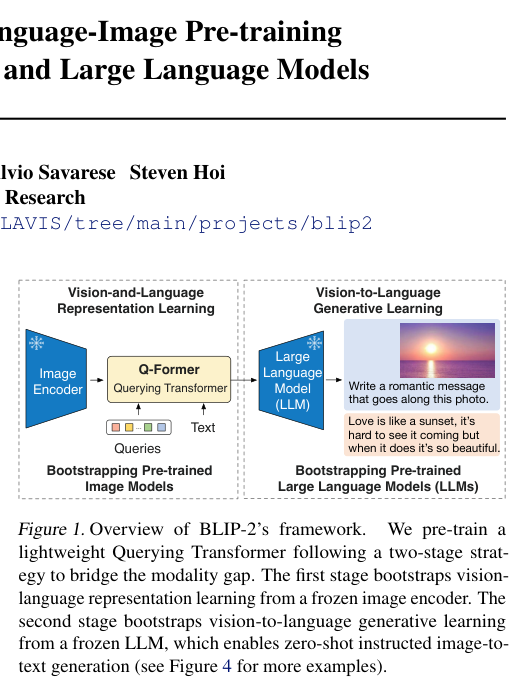
\includegraphics[width=0.75\textwidth,height=0.4\textheight,keepaspectratio]{figures/2301.12597_p1.png}\end{center}

The figure illustrates the two-stage BLIP-2 framework using two dashed boxes connected by a central flow. The first box, "Vision-and-Language Representation Learning," shows an Image Encoder feeding into a Querying Transformer (Q-Former) that produces queries and text; the second box, "Vision-to-Language Generative Learning," shows the Q-Former output feeding into a Large Language Model (LLM) to generate a text description for a given image.

\textbf{Visual Instruction Tuning} — \citep{2304.08485} p.4

\begin{center}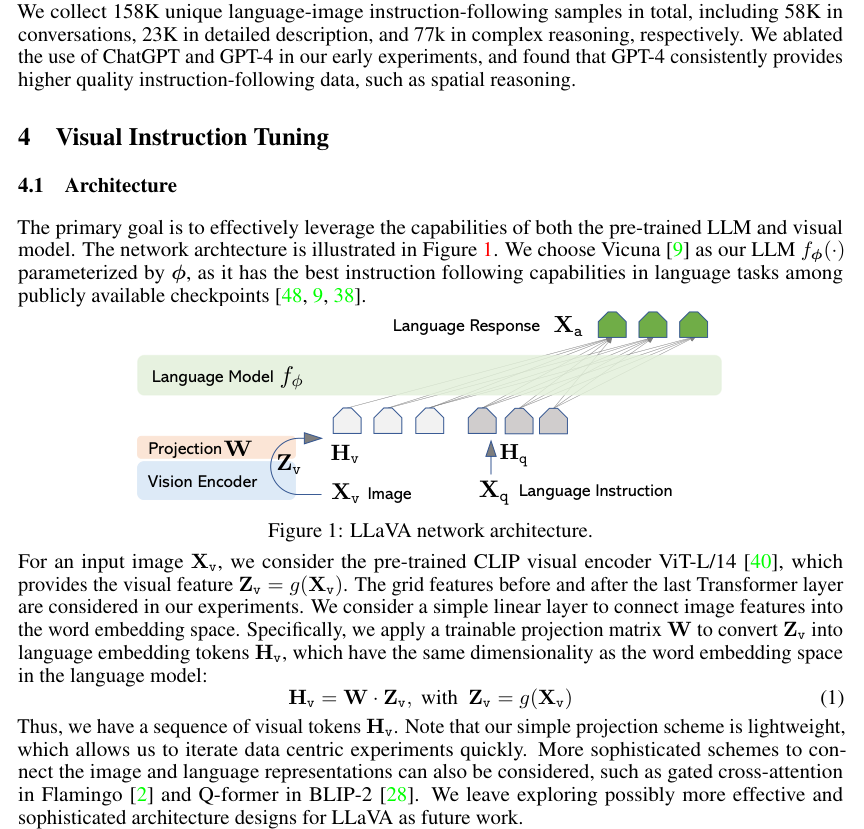
\includegraphics[width=0.75\textwidth,height=0.4\textheight,keepaspectratio]{figures/2304.08485_p4.png}\end{center}

The figure illustrates the LLaVA network architecture, showing a flow from an input image (\$X\_v\$) through a Vision Encoder to a visual feature (\$Z\_v\$), which is then transformed by a projection matrix (\$W\$) into language tokens (\$H\_v\$). These tokens, along with language instruction tokens (\$H\_q\$) derived from an input instruction (\$X\_q\$), are fed into a Language Model (\$f\_\textbackslash{}phi\$) to produce a language response (\$X\_a\$).

**MiniGPT-4: Enhancing Vision-Language Understanding with Advanced Large
  Language Models** — \citep{2304.10592} p.2

\begin{center}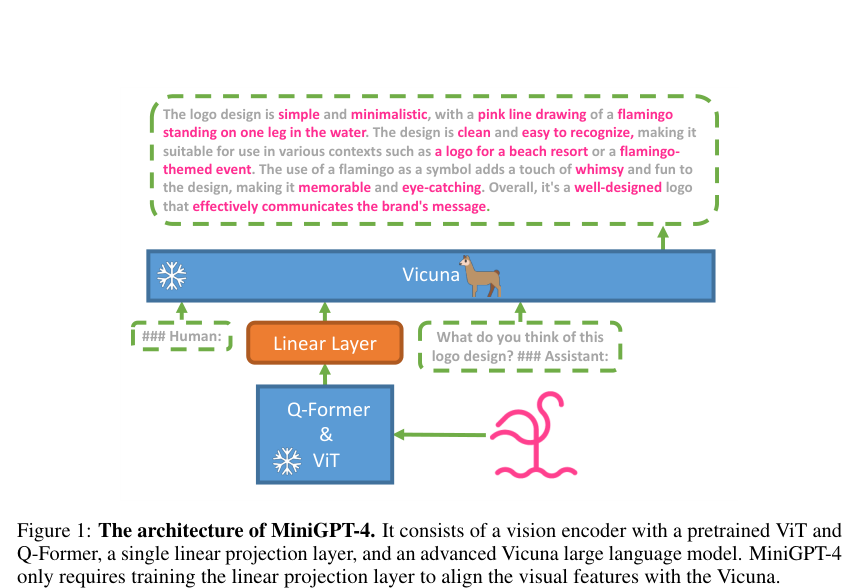
\includegraphics[width=0.75\textwidth,height=0.4\textheight,keepaspectratio]{figures/2304.10592_p2.png}\end{center}

The figure illustrates the MiniGPT-4 architecture through a flowchart of interconnected boxes and text bubbles. It shows a visual encoder (Q-Former \& ViT) feeding into a Linear Layer, which then connects to a Vicuna large language model, with dashed arrows representing a dialogue exchange between a human and an assistant. The diagram conveys how visual information is processed and projected to align with the language model to generate a descriptive text response about a flamingo logo.

\textbf{GPT-4 Technical Report} — \citep{2303.08774} p.3

\begin{center}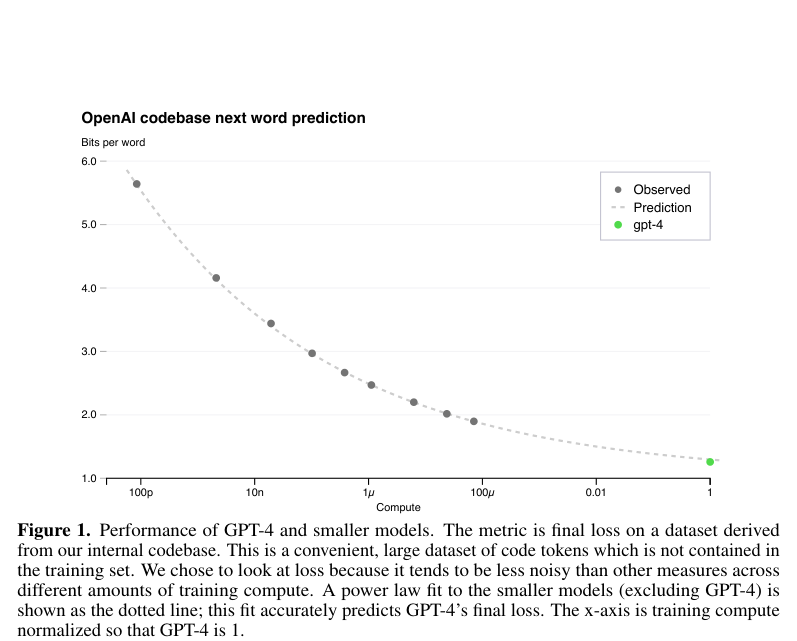
\includegraphics[width=0.75\textwidth,height=0.4\textheight,keepaspectratio]{figures/2303.08774_p3.png}\end{center}

This line graph plots bits per word (y-axis) against compute (x-axis) for next-word prediction on an OpenAI codebase dataset. It displays a series of grey dots representing observed performance for smaller models, a dashed grey line representing a power law prediction fit to those observations, and a single green dot representing GPT-4's performance. The figure conveys that GPT-4's loss aligns with the scaling trends predicted by a power law fit to smaller models.

\textbf{Improved Baselines with Visual Instruction Tuning} — \citep{2310.03744} p.1

\begin{center}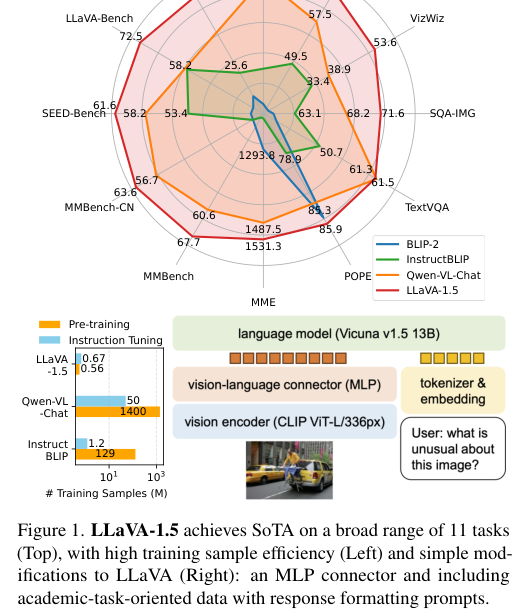
\includegraphics[width=0.75\textwidth,height=0.4\textheight,keepaspectratio]{figures/2310.03744_p1.png}\end{center}

This radar chart compares the performance of LLaVA-1.5 against four baseline models (BLIP-2, InstructBLIP, Qwen-VL-Chat, and POPE) across 11 different evaluation benchmarks. The axes represent various tasks such as MME, MMBench, and VizWiz, with the LLaVA-1.5 model (represented by a thick red line) showing a larger area coverage than the other models, conveying its superior state-of-the-art performance.

\textbf{Sigmoid Loss for Language Image Pre-Training} — \citep{2303.15343} p.3

\begin{center}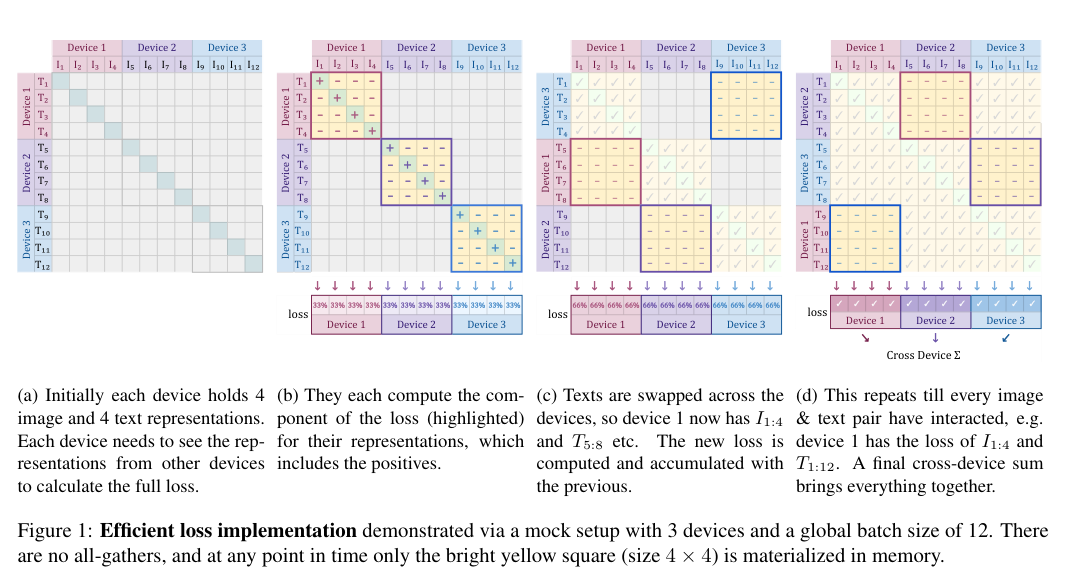
\includegraphics[width=0.75\textwidth,height=0.4\textheight,keepaspectratio]{figures/2303.15343_p3.png}\end{center}

The figure consists of four sequential panels (a–d) using grids of text (\$T\$) and image (\$I\$) indices to illustrate a distributed loss computation process. Each panel uses colored boxes, arrows, and shaded cells to show how local representations are swapped across three devices to compute the full cross-device loss without all-gather operations. The sequence conveys that by iteratively swapping texts and images, the system can accumulate the total loss \$\textbackslash{}Sigma\$ while only materializing a \$4 \textbackslash{}times 4\$ block in memory at any given time.

**mPLUG-Owl: Modularization Empowers Large Language Models with
  Multimodality** — \citep{2304.14178} p.3

\begin{center}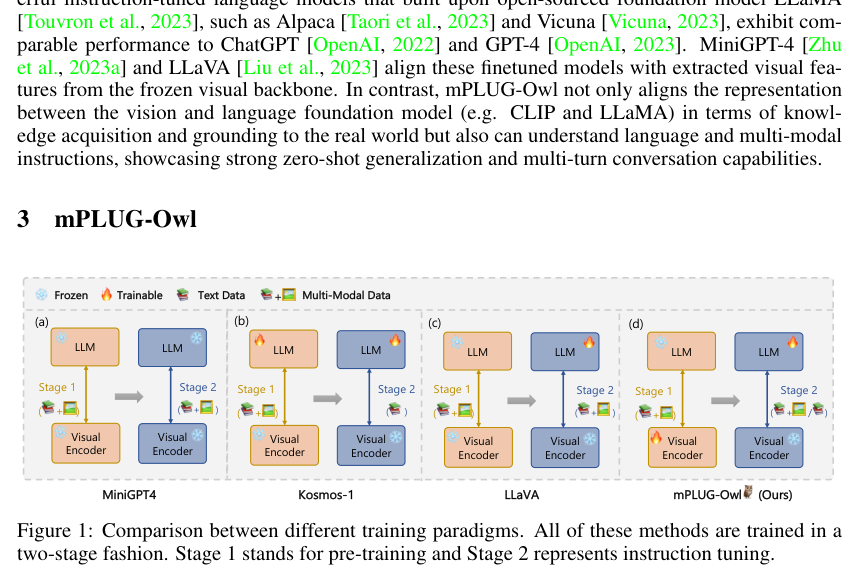
\includegraphics[width=0.75\textwidth,height=0.4\textheight,keepaspectratio]{figures/2304.14178_p3.png}\end{center}

The figure presents a comparative diagram of four training paradigms—MiniGPT4, Kosmos-1, LLaVA, and mPLUG-Owl—using colored boxes to represent LLMs and Visual Encoders, with blue shading indicating frozen components and orange shading indicating trainable components. Arrows labeled "Stage 1" (pre-training) and "Stage 2" (instruction tuning) connect the modules, illustrating how each method transitions from processing text data to multi-modal data. The diagram conveys that while previous methods freeze certain components, the proposed mPLUG-Owl architecture utilizes a specific configuration of trainable and frozen modules across both training stages.

\textbf{Gemini: A Family of Highly Capable Multimodal Models} — \citep{2312.11805} p.3

\begin{center}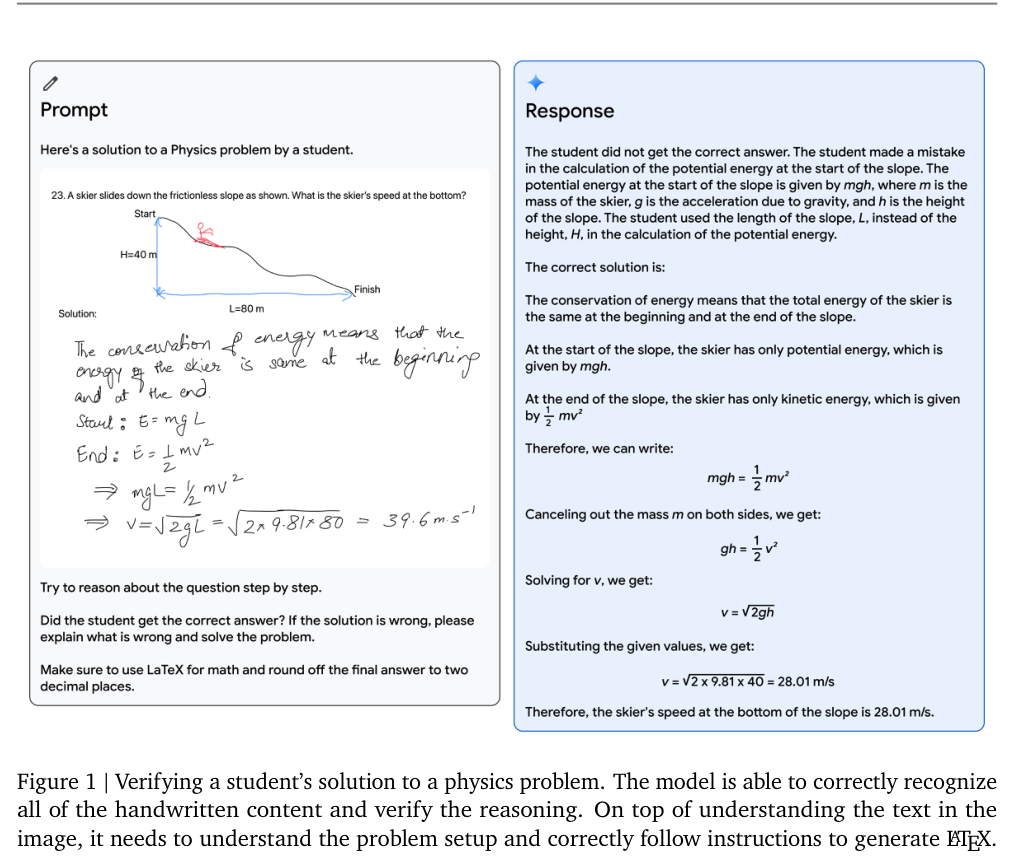
\includegraphics[width=0.75\textwidth,height=0.4\textheight,keepaspectratio]{figures/2312.11805_p3.png}\end{center}

The figure displays a side-by-side comparison of a user prompt and a model response within a chat interface. The prompt contains an image of a handwritten physics problem involving a skier on a slope, accompanied by text instructions to verify the student's reasoning and solution. The response identifies a mistake in the student's potential energy calculation, provides a step-by-step derivation using the conservation of energy, and concludes with the correct answer formatted in LaTeX.

\textbf{EVA-CLIP: Improved Training Techniques for CLIP at Scale} — \citep{2303.15389} p.1

\begin{center}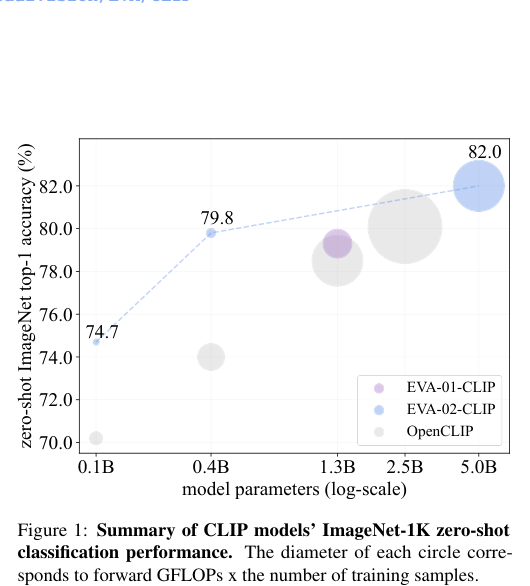
\includegraphics[width=0.75\textwidth,height=0.4\textheight,keepaspectratio]{figures/2303.15389_p1.png}\end{center}

This scatter plot displays the zero-shot ImageNet-1K top-1 accuracy (\%) on the y-axis against the number of model parameters on a log-scale x-axis. The figure uses colored circles of varying sizes to represent different models (EVA-01-CLIP in pink, EVA-02-CLIP in blue, and OpenCLIP in grey), where the circle diameter corresponds to the total training compute (GFLOPs \$\textbackslash{}times\$ number of training samples). The plot conveys that EVA-02-CLIP achieves higher accuracy than OpenCLIP models while utilizing significantly fewer model parameters.

\textbf{Cambrian-1: A Fully Open, Vision-Centric Exploration of Multimodal LLMs} — \citep{2406.16860} p.4

\begin{center}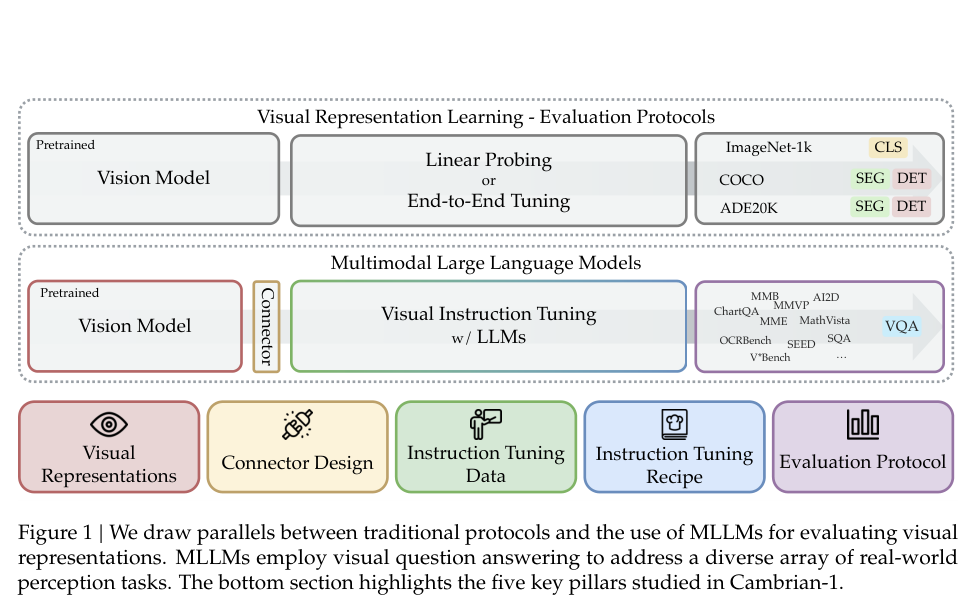
\includegraphics[width=0.75\textwidth,height=0.4\textheight,keepaspectratio]{figures/2406.16860_p4.png}\end{center}

The figure presents a comparative diagram between "Visual Representation Learning - Evaluation Protocols" and "Multimodal Large Language Models," using boxes and arrows to map traditional workflows to modern MLLM architectures. The top section illustrates a pipeline from a pretrained vision model through linear probing or end-to-end tuning to specific tasks like ImageNet-1k (CLS) and COCO/ADE20K (SEG DET). The middle section shows an MLLM pipeline consisting of a pretrained vision model connected to visual instruction tuning with LLMs, leading to various VQA benchmarks. The bottom section consists of five colored boxes representing the key pillars of the Cambrian-1 study: Visual Representations, Connector Design, Instruction Tuning Data, Instruction Tuning Recipe, and Evaluation Protocol.

\textbf{LLaVA-OneVision: Easy Visual Task Transfer} — \citep{2408.03326} p.3

\begin{center}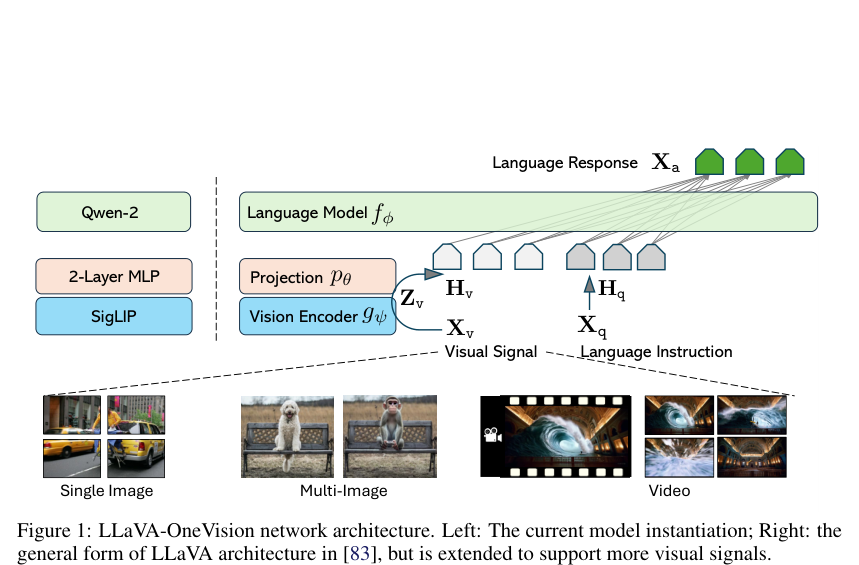
\includegraphics[width=0.75\textwidth,height=0.4\textheight,keepaspectratio]{figures/2408.03326_p3.png}\end{center}

The figure illustrates the LLaVA-OneVision network architecture, comparing a specific model instantiation on the left with a generalized architecture on the right. The diagram uses labeled boxes for components (SigLIP vision encoder, 2-layer MLP projection, and Qwen-2 language model) and arrows to show the flow of data from visual signals (single image, multi-image, or video) and language instructions through the encoder and projection layers into the language model to produce a language response.

\textbf{Language Is Not All You Need: Aligning Perception with Language Models} — \citep{2302.14045} p.1

\begin{center}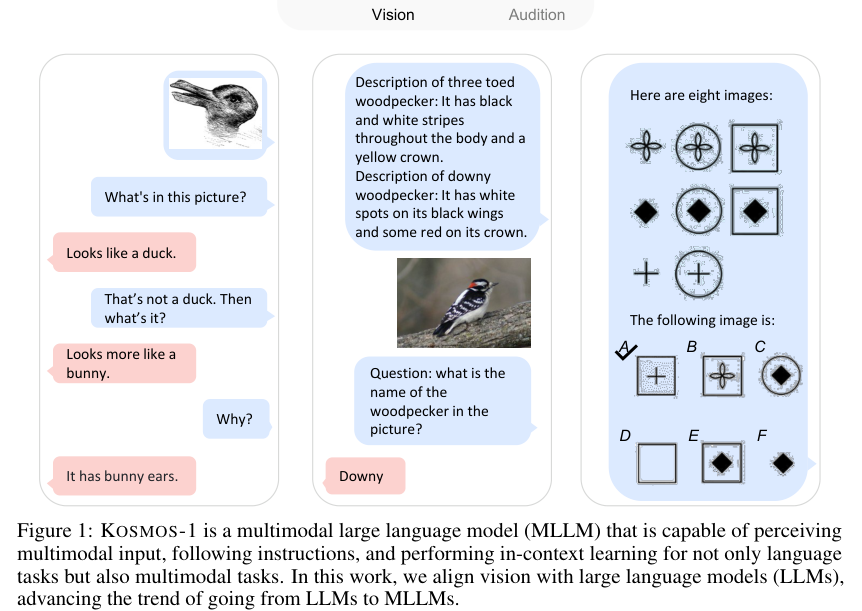
\includegraphics[width=0.75\textwidth,height=0.4\textheight,keepaspectratio]{figures/2302.14045_p1.png}\end{center}

The figure displays three side-by-side panels illustrating the multimodal capabilities of KOSMOS-1 through chat-based interfaces. The left panel shows a visual dialogue where the model identifies a rabbit from an image, the middle panel shows the model identifying a "Downy" woodpecker based on a provided description and image, and the right panel demonstrates in-context learning by asking the model to identify a specific symbol from a set of examples.

**Molmo and PixMo: Open Weights and Open Data for State-of-the-Art
  Vision-Language Models** — \citep{2409.17146} p.2

\begin{center}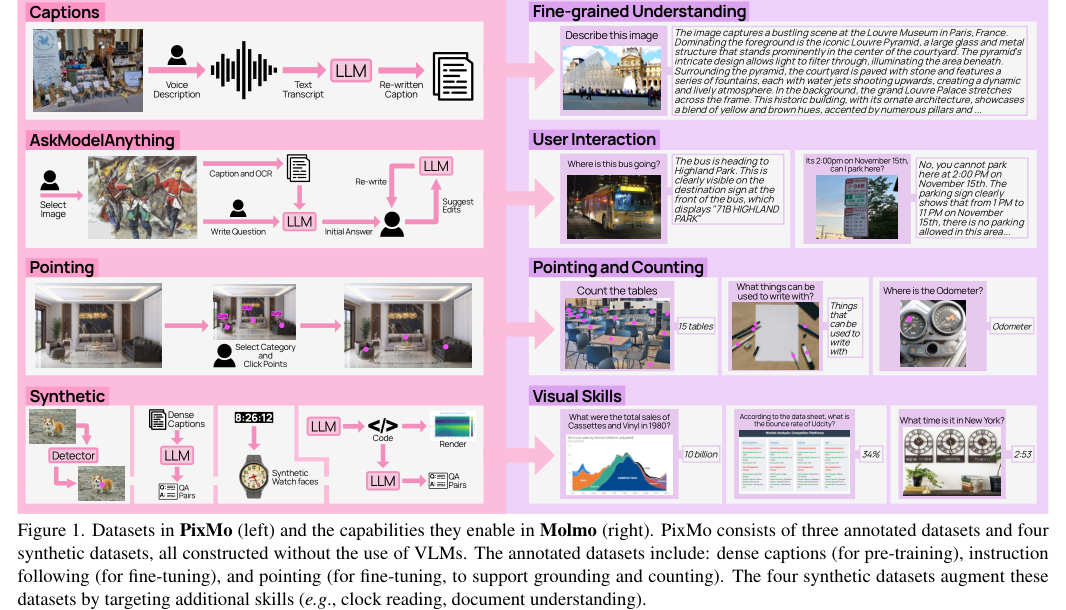
\includegraphics[width=0.75\textwidth,height=0.4\textheight,keepaspectratio]{figures/2409.17146_p2.png}\end{center}

The figure consists of two main panels, PixMo (left) and Molmo (right), organized into four rows of task-specific boxes. The PixMo panel illustrates the data generation pipelines for Captions, AskModelAnything, Pointing, and Synthetic datasets using icons for images, text, and LLM processing blocks. The Molmo panel displays the resulting model capabilities through visual examples of fine-grained understanding, user interaction, pointing and counting, and various visual skills.

\textbf{Grounding Language Models to Images for Multimodal Inputs and Outputs} — \citep{2301.13823} p.1

\begin{center}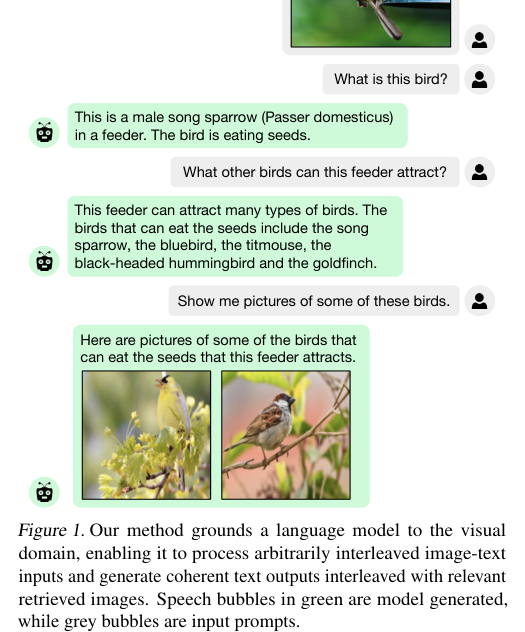
\includegraphics[width=0.75\textwidth,height=0.4\textheight,keepaspectratio]{figures/2301.13823_p1.png}\end{center}

The figure depicts a conversational exchange between a user (gray bubbles) and a language model (green bubbles) regarding an image of a bird. The dialogue shows the model identifying a male song sparrow, listing other birds the feeder might attract, and finally displaying retrieved images of those birds in response to a user request.


\bibliographystyle{unsrtnat}
\bibliography{refs}

\end{document}
